\chapter[Chuyển động của hạt mang điện trong từ trường đều ]{Chuyển động của hạt mang điện trong từ trường đều\footnote{Bài đọc thêm} }
\section{Lý thuyết trọng tâm}
\subsection{Lực tác dụng lên điện tích}
\begin{center}
	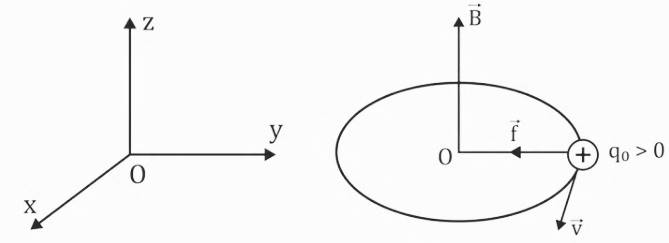
\includegraphics[scale=0.8]{../figs/VN11-PH-27-L-019-2-h82.jpg}
\end{center}

Lực Lo-ren-xơ luôn vuông góc với vận tốc $\vec{v}$, nên lực Lo-ren-xơ đóng vai trò là lực hướng tâm:
\begin{equation}
f=\dfrac{mv^2}{R}=\left|q_0 \right|vB\sin \alpha,
\end{equation}

với $R$ là bán kính cong của quỹ đạo.

\subsection{Quỹ đạo chuyển động của điện tích}

Vì độ lớn của vận tốc không đổi nên bán kính cong $R$ của quỹ đạo không đổi, nói cách khác quỹ đạo là một đường tròn. 


Quỹ đạo của một hạt điện tích trong một từ trường đều, với điều kiện vận tốc ban đầu vuông góc với từ trường, là một đường tròn nằm trong mặt phẳng vuông góc với từ trường, có bán kính:

\begin{equation}
R=\dfrac{mv}{\left| q_0 \right|B},
\end{equation}
trong đó,
\begin{itemize}
	\item $R$ là bán kính quỹ đạo
	\item $m$ là khối lượng hạt,
	\item $v$ là vận tốc hạt,
	\item $q_0$ là điện tích của hạt,
	\item $B$ là cảm ứng từ.
\end{itemize}

\section{Bài tập }
\begin{dang}{Chuyển động của hạt mang điện trong từ trường đều}
\end{dang}
\textbf{Phương pháp giải}

Sử dụng công thức tính bán kính quỹ đạo:
\begin{equation}
R=\dfrac{mv}{\left| q_0 \right|B},
\end{equation}

Từ đó suy ra các giá trị bán kính $R$, khối lượng $m$, điện tích $q_0$, cảm ứng từ $B$, vận tốc $v$.

Công thức tính chu kỳ $T$ và tần số $f$ của hạt mang điện chuyển động quỹ đạo tròn trong từ trường đều:
\begin{equation}
T=\dfrac{2\pi}{\omega}=\dfrac{2\pi v}{R}=\dfrac{2\pi m}{B\left| q_0\right| },
\end{equation}

\begin{equation}
f=\dfrac{1}{T}=\dfrac{B\left| q_0\right| }{2\pi m},
\end{equation}

Định lý biến thiên động năng:

\begin{equation}
W_\text{đ}-W_{\text{đ}_0}=A_\text{ngoại lực},
\end{equation}
trong đó,

\begin{itemize}
	\item $W_\text{đ}$ là động năng của hạt lúc sau,
	\item $W_{\text{đ}_0}$ là động năng của hạt lúc đầu,
	\item $A_\text{ngoại lực}$ là công của ngoại lực.
\end{itemize}

\luuy{Lực Lorentz luôn vuông góc với quỹ đạo chuyển động nên không sinh công.
}

\viduii{2}{

Hạt proton chuyển động theo quỹ đạo tròn bán kính 4 m dưới tác dụng của một từ trường đều $B=\text{2}\cdot 10^{-2}\ \text{T}$. Xác định tốc độ của proton và chu kỳ chuyển động của proton.
\begin{mcq}(2)
	\item $v=\text{2,2}\cdot 10^{6}\ \text{m/s}$, $T=\text{3,3}\cdot 10^{-6}\ \text{s}$.
	\item  $v=\text{7,7}\cdot 10^{6}\ \text{m/s}$, $T=\text{4,4}\cdot 10^{-6}\ \text{s}$.
	\item  $v=\text{7,7}\cdot 10^{6}\ \text{m/s}$, $T=\text{3,3}\cdot 10^{-6}\ \text{s}$.
	\item  $v=\text{2,2}\cdot 10^{6}\ \text{m/s}$, $T=\text{4,4}\cdot 10^{-6}\ \text{s}$.
\end{mcq}}{
\begin{center}
	\textbf{Hướng dẫn giải:}
\end{center}

{Công thức bán kính quỹ đạo: $R=\dfrac{mv}{\left| q \right|B}$.
	
	Suy ra, vận tốc: $v=\dfrac{RB\left| q\right| }{m}$
	
	Các giá trị $R=4\ \text{m}$, $B=\text{2}\cdot 10^{-2}\ \text{T}$, $q=\text{1,6}\cdot 10^{-19}\ \text{C}$, $m=\text{1,67}\cdot 10^{-27}\ \text{kg}$ được thay vào biểu thức.
	
	Suy ra, vận tốc $v=\dfrac{RB\left| q\right| }{m}=\text{7,7}\cdot 10^{6}\ \text{m/s}$.
	
	Chu kỳ của proton: $T=\dfrac{2\pi m}{B\left| q_0\right|}$.
	
	Các giá trị $m=\text{1,67}\cdot 10^{-27}\ \text{kg}$, $B=\text{2}\cdot 10^{-2}\ \text{T}$,  $q=\text{1,6}\cdot 10^{-19}\ \text{C}$, được thay vào biểu thức.

Suy ra, chu kỳ của proton: $T=\dfrac{2\pi m}{B\left| q_0\right|}=\text{3,3}\cdot 10^{-6}\ \text{s}$.

\textbf{	Đáp án: C.}
}}

\viduii{3}{
Hạt electron với vận tốc đầu bằng không được gia tốc qua một hiệu điện thế 600 V. Tiếp đó nó được dẫn vào miền có từ trường đều có vectơ cảm ứng từ $\vec{B}$ vuông góc với $\vec{v}$. Quỹ đạo của electron là đường tròn bán kính $R=5\ \text{cm}$.  Xác định độ lớn cảm ứng từ $B$.

\begin{mcq}(4)
	\item $\text{2,65}\cdot 10^{-3}\ \text{T}$.
	\item $\text{1,65}\cdot 10^{-3}\ \text{T}$.
	\item $\text{3,65}\cdot 10^{-3}\ \text{T}$
	\item $\text{4,65}\cdot 10^{-3}\ \text{T}$.
\end{mcq}}{
\begin{center}
	\textbf{Hướng dẫn giải:}
\end{center}

{ Định lí biến thiên động năng: $W_\text{đ}-W_{\text{đ}_0}=A_\text{ngoại lực}$.
	
	Hay $\dfrac{1}{2}mv^2-0=\left|q \right|U$.
	
	Suy ra $v=\sqrt{\dfrac{2\left| q\right|U }{m}}$.
	
	Các giá trị $q=-\text{1,6}\cdot 10^{-19}\ \text{C}$, $U=\text{600}\ \text{V}$, $m=\text{9,1}\cdot 10^{-31}\ \text{kg}$ được thay vào biểu thức.
	
	Vận tốc $v=\sqrt{\dfrac{2\left| q\right|U }{m}}=\text{14,53}\cdot 10^{6}\ \text{m/s}$.
	
	Công thức bán kính quỹ đạo: $R=\dfrac{mv}{\left| q \right|B}$.
	
	Suy ra, độ lớn cảm ứng từ $B=\dfrac{mv}{R\left| q\right|}$.
	
	Các giá trị $m=\text{9,1}\cdot 10^{-31}\ \text{kg}$, $v=\text{14,53}\cdot 10^{6}\ \text{m/s}$, $R=\text{0,05}\ \text{m}$, $q=-\text{1,6}\cdot 10^{-19}\ \text{C}$ được thay vào biểu thức.
	
	Suy ra, độ lớn cảm ứng từ $B=\dfrac{mv}{R\left| q\right|}=\text{1,65}\cdot 10^{-3}\ \text{T}$.
	
\textbf{Đáp án: B.}
}
}



